\documentclass[Lau, oneside]{sapthesis}%remove "english" for a thesis written in Italian
\graphicspath{ {images/} }
%Bachelor's (laurea triennale) thesis : Lau 
%Master's (laurea specialistica) thesis: LaM 
%PhD's thesis: PhD 
\usepackage[italian]{babel} %use this package for a thesis written in Italian
\usepackage[utf8]{inputenx}
\usepackage{indentfirst}
\usepackage{microtype}
%\usepackage{chemformula}
%\usepackage{setspace}
%\usepackage{yfonts,color}https://www.overleaf.com/project/5e4187442ef81c00013a37ea
%\usepackage{siunitx}
%\usepackage{comment}
%\usepackage{multirow}
%\usepackage{varioref}
%\usepackage[bottom]{footmisc}
%\usepackage{wrapfig}
%\usepackage{float}
%\usepackage{type1cm}
\usepackage{lettrine}
%portare linespread a 1.1-1.3
\linespread{1.4}
%\usepackage{chngcntr}
\usepackage[nottoc, notlof, notlot]{tocbibind}
%\onehalfspacing
%\counterwithout{footnote}{chapter}
\usepackage{hyperref}
\hypersetup{
			hyperfootnotes=true,			
			bookmarks=true,			
			colorlinks=true,
			linkcolor=red,
                        linktoc=page,
			anchorcolor=black,
			citecolor=red,
			urlcolor=blue,
			pdftitle={Sviluppo App},
			pdfauthor={Edoardo Gabrielli},
			pdfkeywords={thesis, sapienza, roma, university}
 }

\title{Sviluppo App}
\author{Edoardo Gabrielli}
\IDnumber{1693726}
\course[]{Informatica}
\courseorganizer{Facolt\`a di Ingegneria dell’Informazione, Informatica e Statistica}
\submitdate{2019/2020}
\copyyear{2020}
\advisor{Prof. Emanuele Panizzi}
\authoremail{gabrielli.1693726@studenti.uniroma1.it}
\examdate{23 marzo 2020}
\examiner{Prof.}

%we refer to http://ctan.mirrorcatalogs.com/macros/latex/contrib/sapthesis/sapthesis-doc.pdf for an exhaustive description of the sapthesis documentclass.


\begin{document}

\frontmatter
\maketitle
\begin{abstract}
Oggetto della tesi è lo sviluppo delle app InfoStud e InfoProf in cui mi sono occupato di risolvere i problemi pre-esistenti e aggiungere nuove funzionalità di entità variabile. Il documento è diviso in tre macro aree: un'introduzione generale alle applicazioni, al processo di sviluppo e agli strumenti utilizzati, poi l'iniziale attività di bug-fixing che comprende anche l'aggiunta di piccole features e infine una parte dedicata allo studio, progettazione ed implementazione dell'apertura di un verbale d'esame.
\end{abstract}

\tableofcontents

\mainmatter
\chapter{Introduzione}
\label{ch:1}

\section{InfoStud e InfoProf}
\label{sec:pres}
L'app InfoStud nasce \textit{n} anni fa dalla necessità degli studenti di avere il sistema InfoStud sviluppato da InfoSapienza su mobile.
Data la natura poco \textit{mobile-friendly} del sistema web, nacque l'app ufficiale sotto il brand di SapienzaApps.

SapienzaApps, sotto il coordinamento del Prof. Emanuele Panizzi, pubblica e mantiene progetti come SeismoCloud e GeneroCity all'interno
del Gamification Lab.

InfoStud è l'app che si rivolge unicamente agli studenti iscritti alla Sapienza e mette a disposizione un parco di funzionalità ampio
che copre le funzioni standard del sistema padre (come visualizzazione e gestione esami) e andando oltre in alcuni casi: il sistema
di gestione dell'orario didattico semi-automatico, la compilazione dei bollettini automatica, la prenotazione dei posti in biblioteca, ecc.

InfoProf, al contrario, è l'app che si rivolge ai professori della Sapienza e vuole essere uno strumento alternativo, e più intuitivo, 
del sistema web. La semplicità di utilizzo dell'app va però analizzata e progettata in modo empirico. Questo studio porta via molto tempo 
al lavoro ed è per questo che gran parte della progettazione si traduce in prototyping e test di usabilità, con eventualmente molteplici
iterazioni. Lo stato dell'arte attualmente è un'app che permette di verbalizzare gli studenti, attivare gli OPIS e cercare le aule.
Queste funzionalità hanno un denominatore in comune: sono casi d'uso in cui l'utente potrebbe non avere il computer quando ha bisogno
di utilizzarle. La verbalizzazione infatti può essere fatta subito dopo un orale, senza dover aspettare di tornare in ufficio e 
registrare i voti di tutti gli studenti. L'OPIS, date le ultime disposizioni, deve essere attivato durante la lezione, ma un utente
potrebbe non voler portare un computer in aula solo per attivare il codice OPIS.

Il mio tirocinio, in larga parte, è stato composto dall'aggiunta di piccole funzionalità richieste dall'utenza o dalla risoluzione di 
problemi: su InfoStud mi sono occupato di migliorare il login, aggiungere un'icona su SmartBiblio per indicare i posti non gestiti
dal sistema, migliorare la dark-mode e aggiungere l'immagine del profilo nel menù laterale. Su InfoProf invece ho lavorato alla
traduzione automatica, anche qui sul login, sul date-picker nella registrazione del voto di un esame e infine sul vero protagonista del 
tirocinio, ovvero l'apertura di un verbale, in cui ho fatto uno studio più approfondito di cui parlerò in \ref{ch:3}.

\section{Perché?}
\label{sec:why}
%trovare articoli scientifici in merito. 
Lo smartphone è ormai uno strumento radicato nella nostra quotidianeità. Sono innumerevoli i modi in cui ha cambiato la nostra vita e la
produttività è uno degli aspetti centrali. Nel settore pubblico l'evoluzione dei sistemi informatici però pecca di una rigorosa analisi 
e progettazione, il che comporta perdite di tempo e difficoltà nell'utilizzo.
Dall'indagine preliminare che ho svolto infatti emerge che alcuni intervistati trovano l'interfaccia web \textit{error-prone}, mentre 
un professore assunto recentemente, ha dichiarato che la piattaforma non è affatto user-friendly e che la logica vorrebbe che ci fosse
un tasto "crea appello", non che debba andarlo a cercare in "verbalizzazione". Anche all'interno del team di sviluppo, quando ci è
stata presentata per la prima volta l'interfaccia, abbiamo faticato a capire come svolgere i task che un professore è tenuto normalmente
a fare. Tolti errori grossolani come l'assegnazione di termini differenti alla stessa cosa [trovare un termine più adatto] 
\textbf{(inserire figura)}, esistono delle criticità che vanno contro la logica comune: se andiamo ad osservare la lista degli insegnamenti,
alla destra di ogni elemento possiamo osservare un numero che rappresenta il numero di \textit{corsi} selezionati accoppiati con quell'
insegnamento. Se selezioniamo il checkbox dell'elemento e andiamo all'interno del sotto-menù, deselezionando tutti i corsi, l'insegnamento
rimarrà selezionato. Una buona interfaccia \textbf{(citare)}, invece, dovrebbe aiutare l'utente ad evitare gli errori.

%citare le statistice del miur riguardo età e numero di docenti della sapienza

%L'approccio che ho avuto quindi è stato quello di capire cosa gli utenti ritengono più importante nell'apertura di un verbale e mettere
%in secondo piano le funzionalità che vengono usate raramente. Vedremo infatti che paradossalmente l'interfaccia web, ai docenti che 
%hanno imparato ad usarla, piace.


\chapter{Metodologie di sviluppo}
\label{ch:2}

\section{Organizzazione}
\label{sec:team}
Il team è composto da studenti impiegati nello sviluppo per circa tre mesi. E' prassi iniziare ad ambientarsi nei progetti attraverso
l'attività di bug-fixing: familiarizzare con il codice e con i colleghi è centrale dato che per molti di noi è la prima esperienza
dentro un progetto di discrete dimensioni e all'interno di un contesto semi-professionale.

La metodologia di sviluppo che si adatta meglio alle nostre esigenze è l'Agile, il quale si basa su un insieme di regole il cui senso
generale è un approccio adatto ai cambiamenti, non fisso e rigoroso, che misura i progressi attraverso codice funzionante e incoraggia 
il rilascio continuo del software per soddisfare l'utente finale. 

Un aspetto fondamentale che si ricollega a questo è l'integrazione
continua del codice prodotto dagli sviluppatori: nel laboratorio utilizziamo GitLab, un sistema di controllo versione che tiene
traccia delle modifiche, segnala i conflitti che possono generarsi dalla modifica simultanea dello stesso file e aiuta a gestire i compiti 
del singolo sviluppatore.
Ad ogni \textit{merge request}, le modifiche apportate al codice sono revisionate da un controllo umano che garantisce la qualità del codice.
Se infatti lo stile non è coerente con il resto del progetto, se ci sono bug introdotti dalle modifiche o altri problemi, la merge request 
viene respinta.

\section{Tecnologie utilizzate}
\label{sec:tech}
Per sviluppare il front-end delle app utilizziamo Ionic Framework v3, che è basato su AngularJS. Ionic permette di utilizzare tecnologie
web per creare interfacce secondo gli standard di Android e iOS. Il vantaggio dell'uso di Angular è che il codice non va adattato ad alcuna
piattaforma, inoltre per chiunque abbia già una discreta conoscenza della programmazione web è immediato iniziare a programmare. Tutto
ciò velocizza molto la scrittura di una UI, ma bisogna fare dei compromessi: l'interfaccia non segue diligentemente gli standard imposti
dal Material Design o dall'iOS UI Design perché deve adattarsi ad entrambe le piattaforme. Un'altra criticità è che di fatto l'app è
un'interfaccia web con caratteristiche \textit{app-like}, ovvero una Progressive Web App sviluppata in Angular. 
Il ruolo di Ionic è fornire gli elementi dei vari standard di design già fatti e di integrare anche le funzionalità native attraverso
Ionic Native o Cordova. Ciò significa che le prestazioni ne risentono ripetto ad un'app nativa. Inoltre ad oggi Ionic è alla versione 5,
ma è impossibile aggiornare i progetti senza andare a creare dei conflitti che vanno risolti manualmente, vista la mole di codice che è
stato scritto quindi, siamo costretti a rimanere ad una versione di qualche anno fa, all'occorenza programmando manualmente le novità
introdotte dagli standard.

InfoStud ed InfoProf sono progettati seguendo un pattern architetturale loro. L'idea generale è quella di tenere separate le responsabilità
di ogni componente. Ciò si traduce sinteticamente in:

\begin{itemize}
	\item Model: rappresentano le classi, contiengono i dati dell'applicazione a cui si accede attraverso i metodi che forniscono;
	\item View: la view accede ai dati forniti dai modelli e li presenta all'utente, inoltre comunica con i controller e i provider;
	\item Controller: il controller risponde alle azioni dell'utente intercettate dalla view e si occupa soltanto della logica di business, a volte comunica con i provider;
	\item Provider: di fatto "fornisce" i dati. Ha il compito di utilizzare le API e consegnare i dati alla view attraverso i model.
\end{itemize}

\begin{figure}[h]
	\caption{Schema del funzionamento del pattern utilizzato da InfoStud e InfoProf.}
	\centering
	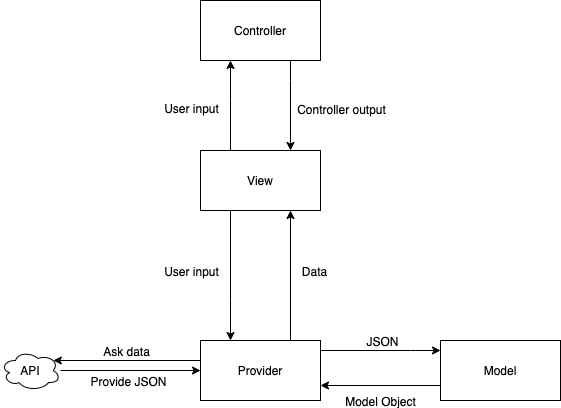
\includegraphics[width=0.8\textwidth]{arch-pattern-img}
	\label{fig:pattern}
\end{figure}

I vantaggi dell'utilizzo di questo modello è quello di separare la logica di presentazione, quella di business e quella di accesso ai dati
in entità distinte tra loro in modo da favorire il lavoro di gruppo. Inoltre, essendo Angular un framework che impone una separazione in moduli del codice [citare], una divisione
così fatta incoraggia il riuso del codice ovviamente. %fare diagramma di sequenza e un esempio

%Tra ch 1 e 2 bisognerebbe aggiungere altre 8 pagine, magari apliare la descrizione delle issues


\chapter{Progettazione}
\label{ch:3}
%inserire diagramma di flusso di come viene fatta la progettazione (nf -> protoryping -> test -> repeat)
L'attività di progettazione consiste nel trovare i bisogni dell'utente attraverso delle domande rivolte agli stessi, costruire un prototipo che rispecchi ciò che è emerso dalle domande, eseguire dei test di usabilità sul prototipo e, a seconda delle criticità, emerse dai test modificare il prototipo e ripetere i test finchè si è trovata un'interfaccia che funzioni per gran parte degli utenti.

\section{Need-finding}
\label{sec:nf}
La prima cosa che ho fatto è capire quali sono i bisogni dell'utente. Non avendo mai utilizzato InfoStud docenti, il primo approccio al sistema è stato insieme al Prof. Panizzi che mi ha mostrato il processo di apertura di un verbale d'esame, le varie funzionalità già esistenti e i dati richiesti nel form che il docente è tenuto a compilare. Da questa dimostrazione sono emerse delle criticità: per un utente inesperto come me è difficile prendere confidenza con l'interfaccia in quanto spesso vengono utilizzati diversi termini per rappresentare lo stesso concetto, c'è una lista molto grande di insegnamenti da poter selezionare e bisogna prestare attenzione a quali sono quelli che si selezionano perchè in alcuni casi il sistema potrebbe restituire un errore. Inoltre l'interfaccia non spiega come inserire il giorno dell'esame (quello che effetivamente gli studenti vedono in fase di prenotazione), bisogna chiederlo a chi già ne è a conoscenza.

Essendomi fatto un'idea delle criticità dell'interfaccia attuale, ho creato un sondaggio inviando via email le seguenti domande:

\begin{enumerate}
	\item Se tiene più di un corso, preferisce aprire un verbale unico o aprirne uno per ogni corso che tiene? 
	\item Trova confusionario il processo di apertura di un verbale? Perché?
	\item Quanto tempo prima dalla data dell’esame apre il verbale?
	\item Quanto tempo dà agli studenti per prenotarsi?
	\item E quanti giorni prima, dal giorno dell’esame, chiude le prenotazioni? 
\end{enumerate}

Il sondaggio ha solo una domanda aperta, tra l'altro opzionale, in quanto volevo rendere il sondaggio molto corto in modo da aumentare 
le possibilità di risposta. Per coloro che volessero dedicarmi più tempo ho invece chiesto di argomentare in modo da avere risposte
più complete, infatti a fine email ho incoraggiato ad argomentare le risposte il più possibile.

La prima domanda è stata fatta per capire come gestiscono la lista degli insegnamenti: la lista sull'app infatti è difficile da gestire
vista la sua lunghezza. Quindi se la maggior parte dei professori sceglie di selezionare tutto, potrei sintetizzarla in qualche modo.
La seconda ha un carattere generale, che mira a scoprire qualcosa di più da parte dell'utente.
Le domande dalla 3 alla 5 invece servono a capire se esistono dei vincoli nella scelta delle date per cercare di automatizzare il processo.

Gli intervistati sono 60, presi casualmente in vari dipartimenti dell'ateneo in modo di avere un campione più eterogeneo possibile.
I professori che hanno invece risposto sono stati 19.

\subsection{Verbale unico o uno per ogni corso?}

Come vediamo dall'immagine \ref{fig:d-i} la maggioranza degli intervistati preferisce aprire un verbale per ogni insegnamento.

\begin{figure}[h]
	\caption{Grafico delle risposte date alla prima domanda.}
	\centering
	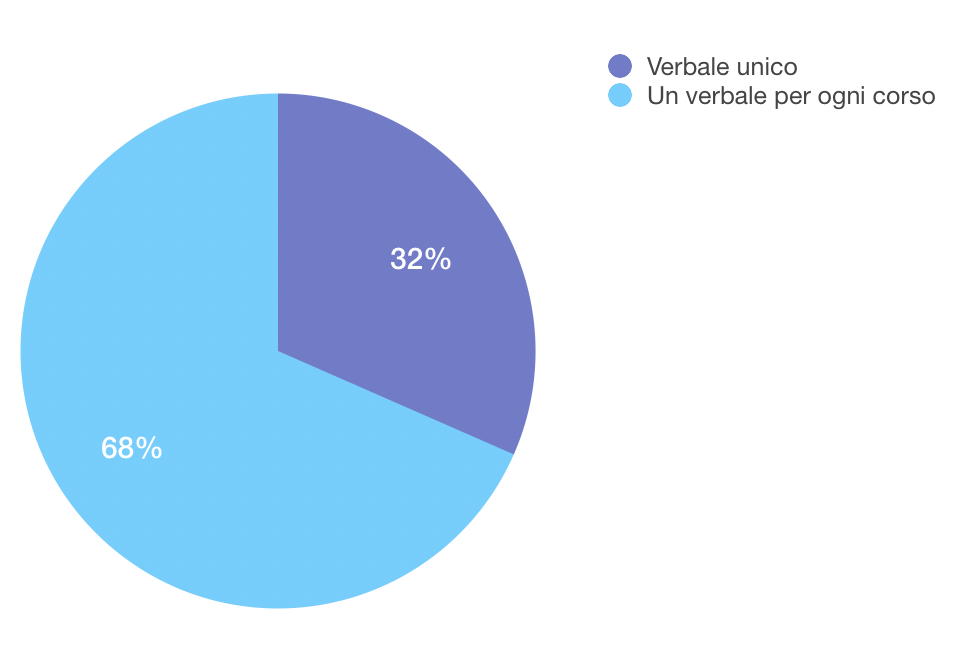
\includegraphics[width=0.6\textwidth]{d-i}
	\label{fig:d-i}
\end{figure}

\subsection{Trova confusionario il processo di apertura di un verbale?}
Qui i risultati sono un po' sorprendenti perchè la maggioranza sostiene che non ci siano grossi problemi, sebbene comunque una percentuale non trascurabile abbia risposto il contrario. Ciò potrebbe essere imputabile al fatto che per molti anni sono stati abituati a questo sistema ed hanno imparato ad utilizzarlo agevolmente, con degli escamotage. Uno fra tutti è quello di utilizzare la funzionalità del "Duplica appello", che di fatto copia un appello già creato. L'utente la utilizza per non dover selezionare nuovamente gli insegnamenti (cambiando dunque le date e le note), ma il nome della funzionalità di fatto suggerisce un altro tipo di utilizzo. Vedremo in seguito come si è trovata una soluzione più elegante a questo problema.

\begin{figure}[h]
	\caption{Grafico delle risposte date alla seconda domanda.}
	\centering
	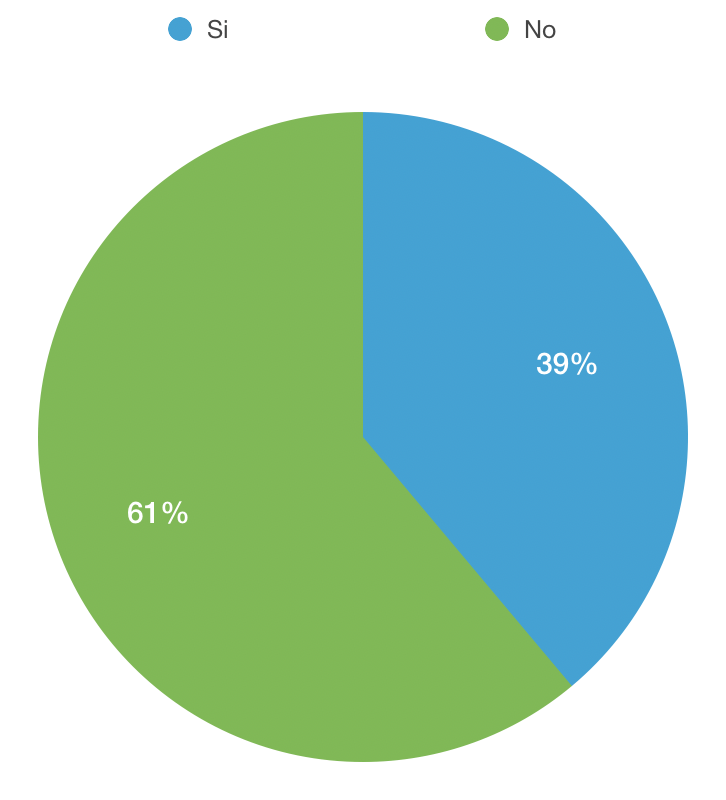
\includegraphics[width=0.4\textwidth]{d-ii}
	\label{fig:d-ii}
\end{figure}

\subsection{Quanto tempo prima dalla data dell’esame apre il verbale?}

\begin{figure}[h]
	\caption{Grafico delle risposte date alla terza domanda.}
	\centering
	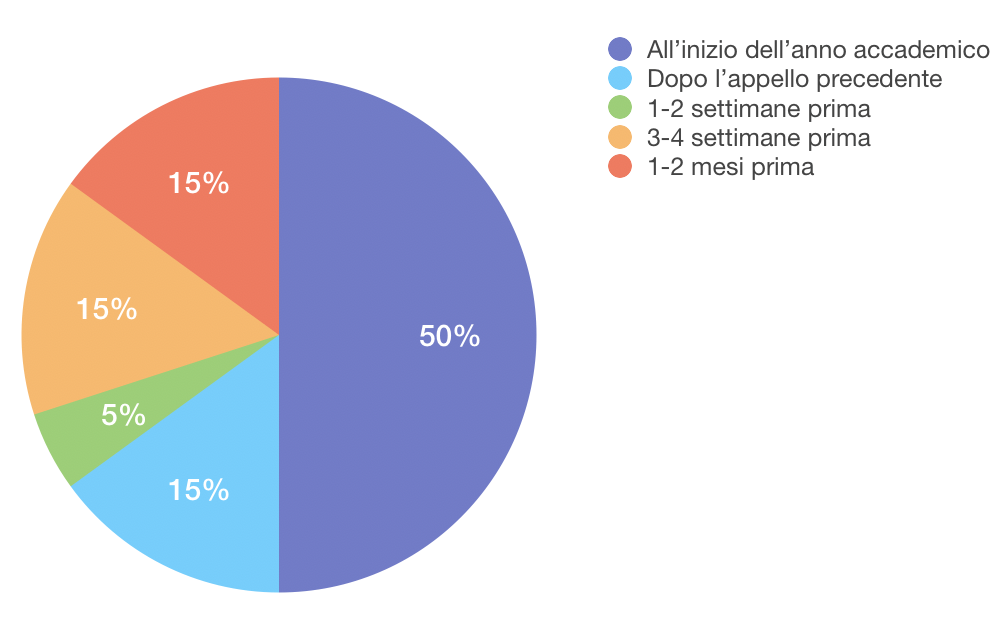
\includegraphics[width=0.8\textwidth]{d-iii}
	\label{fig:d-iii}
\end{figure}

\subsection{Quanto tempo dà agli studenti per prenotarsi?}

\begin{figure}[h]
	\caption{Grafico delle risposte date alla quarta domanda.}
	\centering
	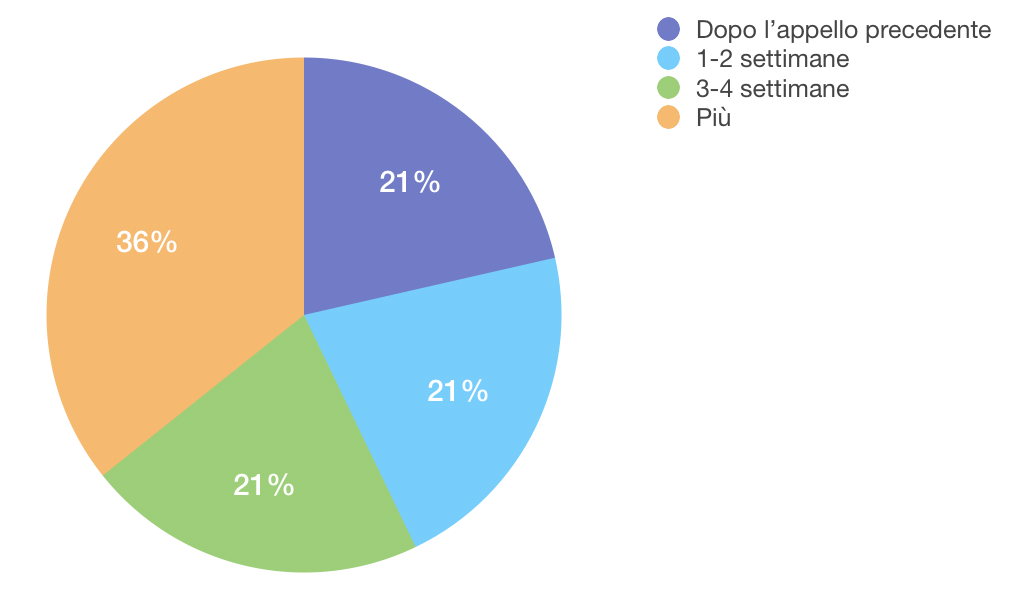
\includegraphics[width=0.8\textwidth]{d-iv}
	\label{fig:d-iv}
\end{figure}

\subsection{E quanti giorni prima, dal giorno dell’esame, chiude le prenotazioni? }

\begin{figure}[h]
	\caption{Grafico delle risposte date alla quinta domanda.}
	\centering
	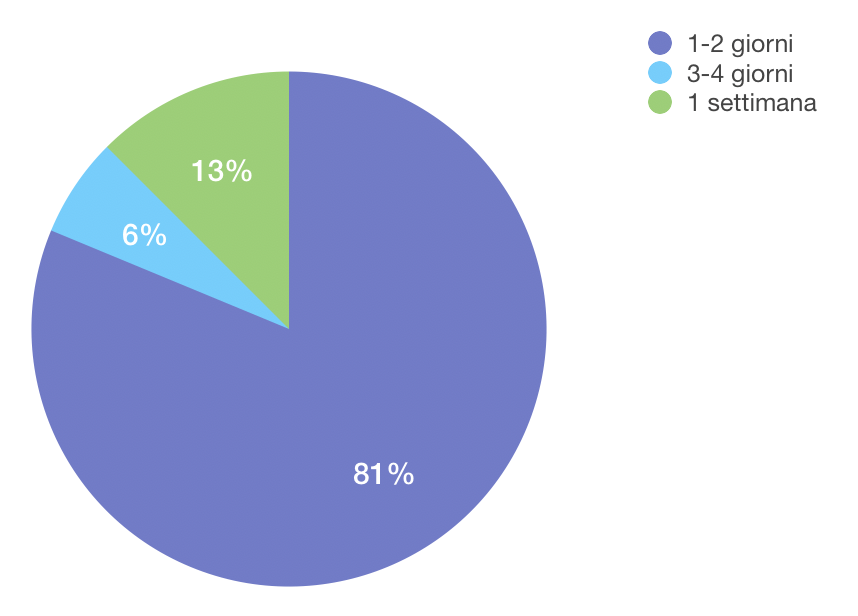
\includegraphics[width=0.7\textwidth]{d-v}
	\label{fig:d-v}
\end{figure}


\section{Progettazione della UI}
\label{sec:ui}
%citare "Developing SMASH"

\section{Implementazione}
\label{sec:dev}
%inserire qualche snippet e magari parlare dei limiti tecnologici di ionic e come li ho superati


\chapter{Concluzioni}
\label{ch:4}

\backmatter
\phantomsection
\begin{thebibliography}{17}

\bibitem{ref:mit}
Tratto da MIT:
\url{http://web.mit.edu/6.813/www/sp18/classes/09-more-learnability/#consistency}

\end{thebibliography}

\end{document}